\chapter{Monads}
\label{chap:monads}

\epigraph{
  La Monade, dont nous parlerons icy, n'est autre chose qu'une
  substance simple...
}{---\textcite[1]{leibniz-1714}}

%% In this chapter we explore monads and their relation to monads in
%% Haskell and Agda.

In Haskell, given two types \texthaskell{a} and \texthaskell{b}, the
Cartesian product\footnote{This definition is adapted from
  \parencite{weisstein-cartesian}.} of a list \texthaskell{xs} of
elements of type \texthaskell{a} and a list \texthaskell{ys} of
elements of type \texthaskell{b} is defined to be the list of tuples
\texthaskell{(x,y)} of type \texthaskell{(a,b)} for which
\texthaskell{x} belongs to \texthaskell{xs} and \texthaskell{y}
belongs to \texthaskell{ys}, that is, using a list comprehension:
\begin{codehaskell}
cartesian :: [a] -> [b] -> [(a,b)]
cartesian xs ys = [(x,y) | x <- xs, y <- ys]
\end{codehaskell}
or, equivalently, desugaring the list comprehension,
\begin{codehaskell}
cartesian xs ys = xs >>= \ x -> ys >>= \ y -> return (x,y)
\end{codehaskell}
which should be clarified by Examples \ref{ex:monad-list-haskell} and
\ref{ex:triple-list-haskell}. This is but one simple example to show
that ``a monad is often an obvious and useful tool to help solve a
problem'' \parencite[325]{osullivan-2008} and that ``many common
programming patterns have a monadic structure''
\parencite[328]{osullivan-2008}.

\todo{What follows is an idea for the introduction, but it is not
  ready.}

\todo{Remember to cite moggi-1989 to say that a computation is the
  denotation of a program and a notion of a computation is a
  qualitative description of a computation.}

In \parencite{moggi-1991}, category theory is taken as a general
theory of functions and develop on top a \emph{categorical semantics
  of computations} based on monads \parencite[56]{moggi-1991}.

The basic idea behind the categorical semantics below is that, in
order to interpret a programming language in a category \cat{C}, we
distinguish the object $a$ of values (of type $a$) from the object
$\funcO{T}(a)$ of computations (of type $a$), and take as denotations
of programs (of type $a$) the \emph{elements} of $\funcO{T}(a)$. In
particular, we identify the type $a$ with the object of values (of
type $a$) and obtain the object of computations (of type $a$) by
applying an unary type-constructor \funcO{T} to $a$. We call \funcO{T}
a \emph{notion of computation}, since it abstracts away from the type
of values computations may produce. There are many choices for
$\funcO{T}(a)$ corresponding to different notions of computations
\parencite[57--58]{moggi-1991}.

Rather than focusing on a specific \funcO{T}, we want to find the
general properties common to all notions of computation; therefore we
impose as the only requirement that \emph{programs} should form a
category. Such a requirement amounts to saying that \funcO{T} is part
of a Kleisli triple and that the category of programs is the Kleisli
category for such a triple \parencite[58]{moggi-1991}.

Kleisli triples are just an alternative description for monads.
Although the former are easy to justify from a computational
perspective, the latter are more widely used in the literature on
category theory and have the advantage of being defined only in terms
of functors and natural transformations, which make them more suitable
for abstract manipulation \parencite[60]{moggi-1991}.

\section{Monads}
\label{sec:monads}

...

\todo{(Idea) Notions of computation as triples.}

\todo{Introduce Example \ref{ex:notions-computation}.}

\begin{examples}
  \label{ex:notions-computation}

  %% \parencite[58]{moggi-1991}

  Notions of computation:
  \begin{itemize}
  \item
    \emph{Partiality}
  \item
    \emph{Nondeterminism}
  \item
    \emph{Side effects}
  \item
    \emph{Exceptions}
  \item
    \emph{Continuations}
  \item
    \emph{Interactive input}
  \item
    \emph{Interactive output}
  \end{itemize}
\end{examples}

\subsection*{Monads}

As mentioned earlier \todo{Where?}, monads in Haskell and Agda
correspond to triples. However, monads are more widely used in
category theory and more suitable for abstract manipulation because
they are defined only in terms of functors and natural transformations
\parencite[60]{moggi-1991}.

\todo{Note about the identity natural transformation}
\todo{Note about the two equality lines in the second commutative diagram above.}

\begin{definition}
  \label{def:monad}

  %% \parencite[137]{maclane-1998}

  Let \cat{C} be a category. A \emph{monad}
  \begin{equation}
    \label{eq:monad}
    \mon{T} = (\func{T}, \nat{\eta}, \nat{\mu})
  \end{equation}
  in \cat{C} consists of an endofunctor
  \begin{equation}
    \label{eq:monad-}
    \func{T}: \cat{C} \to \cat{C}
    \text{,}
  \end{equation}
  together with two natural transformations\footnote{Whenever a
    natural transformation is mentioned, its naturality is implicitly
    mentioned as well. See Definition \ref{def:natural}.}
  \begin{equation}
    \label{eq:monad-unit}
    \nat{\eta}: \func{I} \to \func{T}: \cat{C} \to \cat{C}
  \end{equation}
  and
  \begin{equation}
    \label{eq:monad-multiplication}
    \nat{\mu}: \func{T \comp T} \to \func{T}: \cat{C} \to \cat{C}
    \text{,}
  \end{equation}
  called \emph{unit} and \emph{multiplication} of the monad,
  respectively, such that, for all objects $a \in \catO{C}$,
  \begin{equation}
    \label{eq:monad-associativity}
    \natO{\mu}{a} \comp \natO{\mu}{\funcO{T}(a)} = \natO{\mu}{a} \comp \funcM{T}(\natO{\mu}{a})
    \text{,}
  \end{equation}
  \begin{equation}
    \label{eq:monad-unity-left}
    \natO{\mu}{a} \comp \natO{\eta}{\funcO{T}(a)} = \idO{\funcO{T}(a)}
    \text{,}
  \end{equation}
  and
  \begin{equation}
    \label{eq:monad-unity-right}
    \natO{\mu}{a} \comp \funcM{T}(\natO{\eta}{a}) = \idO{\funcO{T}(a)}
    \text{,}
  \end{equation}
  that is, such that the diagrams in Figures
  \ref{fig:monad-associativity} and \ref{fig:monad-unity} are
  commutative.
  \begin{figure}[htbp]
    \begin{center}
      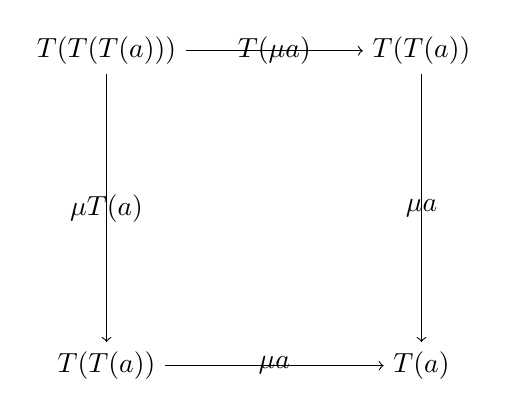
\begin{tikzpicture}[node distance=4cm]
        \node (ttt a)                  {$\funcO{T}(\funcO{T}(\funcO{T}(a)))$};
        \node (tt a1) [right of=ttt a] {$\funcO{T}(\funcO{T}(a))$};
        \node (tt a2) [below of=ttt a] {$\funcO{T}(\funcO{T}(a))$};
        \node (t a)   [right of=tt a2] {$\funcO{T}(a)$};

        \draw [->] (ttt a) to node        {$\funcM{T}(\natO{\mu}{a})$} (tt a1);
        \draw [->] (ttt a) to node [swap] {$\natO{\mu}{\funcO{T}(a)}$} (tt a2);
        \draw [->] (tt a1) to node        {$\natO{\mu}{a}$}            (t a);
        \draw [->] (tt a2) to node [swap] {$\natO{\mu}{a}$}            (t a);
      \end{tikzpicture}
    \end{center}
    \caption{Monadic associativity.}
    \label{fig:monad-associativity}
  \end{figure}
  \begin{figure}[htbp]
    \begin{center}
      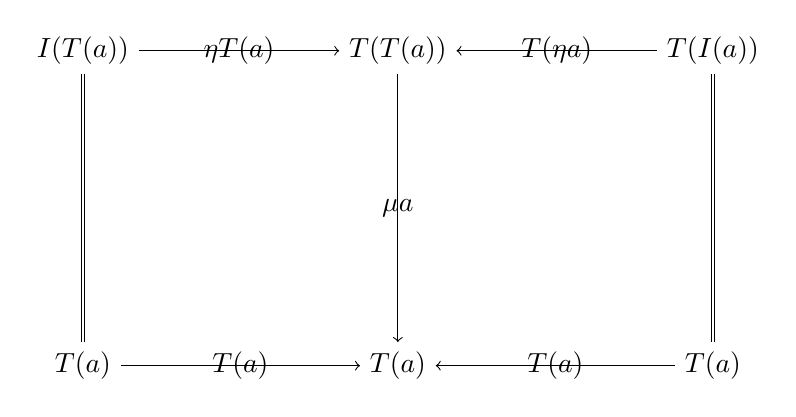
\begin{tikzpicture}[node distance=4cm]
        \node (it a)                 {$\funcO{I}(\funcO{T}(a))$};
        \node (tt a) [right of=it a] {$\funcO{T}(\funcO{T}(a))$};
        \node (ti a) [right of=tt a] {$\funcO{T}(\funcO{I}(a))$};
        \node (t a1) [below of=it a] {$\funcO{T}(a)$};
        \node (t a2) [right of=t a1] {$\funcO{T}(a)$};
        \node (t a3) [right of=t a2] {$\funcO{T}(a)$};

        \draw [->] (it a) to node        {$\natO{\eta}{\funcO{T}(a)}$} (tt a);
        \draw [->] (ti a) to node [swap] {$\funcM{T}(\natO{\eta}{a})$} (tt a);

        \draw [double] (it a) to                        (t a1);
        \draw [->]     (tt a) to node {$\natO{\mu}{a}$} (t a2);
        \draw [double] (ti a) to                        (t a3);

        \draw [->] (t a1) to node [swap] {$\idO{\funcO{T}(a)}$} (t a2);
        \draw [->] (t a3) to node        {$\idO{\funcO{T}(a)}$} (t a2);
      \end{tikzpicture}
    \end{center}
    \caption{Monadic unity.}
    \label{fig:monad-unity}
  \end{figure}

  Additionally, since \nat{\eta} and \nat{\mu} are natural
  transformations, then, for all morphisms $f: a \to \funcO{T}(b) \in
  \catM{C}$,
  \begin{equation}
    \label{eq:monad-naturality-unit}
    \natO{\eta}{\funcO{T}(b)} \comp f = \funcM{T}(f) \comp \natO{\eta}{a}
  \end{equation}
  and
  \begin{equation}
    \label{eq:monad-naturality-multiplication}
    \natO{\mu}{\funcO{T}(b)} \comp \funcM{T}(\funcM{T}(f)) = \funcM{T}(f) \comp \natO{\mu}{a}
    \text{,}
  \end{equation}
  or, equivalently, the diagrams in Figures
  \ref{fig:monad-naturality-unit} and
  \ref{fig:monad-naturality-multiplication} are commutative.
  \begin{figure}[htbp]
    \begin{center}
      \begin{tikzpicture}[node distance=4cm]
        \node (f a)                {$a$};
        \node (f b) [below of=f a] {$\funcO{T}(b)$};
        \node (g a) [right of=f a] {$\funcO{T}(a)$};
        \node (g b) [below of=g a] {$\funcO{T}(\funcO{T}(b))$};

        \draw [->] (f a) to node [swap] {$f$}            (f b);
        \draw [->] (g a) to node        {$\funcM{T}(f)$} (g b);

        \draw [->] (f a) to node        {$\natO{\eta}{a}$}            (g a);
        \draw [->] (f b) to node [swap] {$\natO{\eta}{\funcO{T}(b)}$} (g b);
      \end{tikzpicture}
    \end{center}
    \caption{Naturality of the \nat{\eta} natural transformation.}
    \label{fig:monad-naturality-unit}
  \end{figure}
  \begin{figure}[htbp]
    \begin{center}
      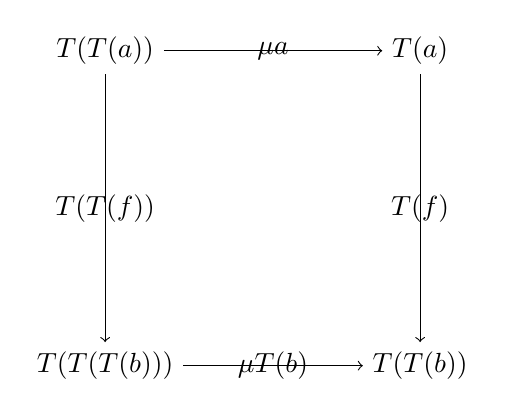
\begin{tikzpicture}[node distance=4cm]
        \node (f a)                {$\funcO{T}(\funcO{T}(a))$};
        \node (f b) [below of=f a] {$\funcO{T}(\funcO{T}(\funcO{T}(b)))$};
        \node (g a) [right of=f a] {$\funcO{T}(a)$};
        \node (g b) [below of=g a] {$\funcO{T}(\funcO{T}(b))$};

        \draw [->] (f a) to node [swap] {$\funcM{T}(\funcM{T}(f))$} (f b);
        \draw [->] (g a) to node        {$\funcM{T}(f)$}            (g b);

        \draw [->] (f a) to node        {$\natO{\mu}{a}$}            (g a);
        \draw [->] (f b) to node [swap] {$\natO{\mu}{\funcO{T}(b)}$} (g b);
      \end{tikzpicture}
    \end{center}
    \caption{Naturality of the \nat{\mu} natural transformation.}
    \label{fig:monad-naturality-multiplication}
  \end{figure}
\end{definition}

\begin{remark}
  \label{re:monad-monoid}

  Formally, the definition of a monad is like that of a monoid $M$, as
  described in Example \ref{ex:monoid}. The set $M$ of
  elements of the monoid is replaced by the endofunctor \func{T} from
  \cat{C} to \cat{C}, while the cartesian product $\times$ of two sets
  is replaced by composite of two functors, the binary operation $\mu:
  M \times M \to M$ of multiplication by
  \eqref{eq:monad-multiplication} and the unit (identity) element
  $\eta: I \to M$ by \eqref{eq:monad-unit}. We shall thus call $\eta$
  the unit and $\mu$ the multiplication of the monad $T$; the diagram
  in Figure \ref{fig:monad-associativity} is then the associative law
  for the monad, while the diagrams in Figure \ref{fig:monad-unity}
  express the left and right unit laws, respectively. Thus, a monad in
  \cat{C} is just a monoid in the category of endofunctors of \cat{C},
  with product $\times$ replaced by composition of endofunctors and
  unit set replaced by the identity endofunctor
  \parencite[138]{maclane-1998}.

\end{remark}

\todo{\nat{\mu} is associative, and \nat{\eta} is a two-sided unit
  for \nat{\mu}.}

\begin{terminology}
  \label{ter:monad}

  Although the common term for monads is monad, alternatives
  include standard construction, which is the original term
  \parencite[30]{manes-1976}, algebraic theory in monoid form
  \parencite[29]{manes-1976}, and triple
  \parencites[83]{barr-2005}[372]{barr-wells-2012}.
  %% , which seems to be the only current alternative.
  We choose monad because of Remark
  \ref{re:monad-monoid} and reserve triple for effectively
  distinguishing between monads and triples, as explained in page
  \pageref{ter:triple}.

\end{terminology}

\begin{example}
  \label{ex:monad-identity}

  The identity or trivial monad is just a reformulation of the
  identity functor for a given category. Compare the following example
  with Example \ref{ex:triple-identity}.

  Given a category \cat{C}, its identity function
  \eqref{eq:category-identity} and its identity endofunctor (Example
  \ref{ex:functor-identity}) yield a monad
  \begin{equation*}
    \mon{I} = (\func{I}, \id, \id)
  \end{equation*}
  in \cat{C}, called the identity monad in \cat{C}.

  \begin{proof}

    Equations \eqref{eq:monad-associativity},
    \eqref{eq:monad-unity-left}, and \eqref{eq:monad-unity-right} hold
    by \eqref{eq:category-identity}, and
    \eqref{eq:monad-naturality-unit} and
    \eqref{eq:monad-naturality-multiplication} hold because \nat{\id}
    is a natural transformation, as demonstrated in Example
    \ref{ex:natural-identity}.

  \end{proof}

\end{example}

\subsection*{Kleisli triples}

As stated above, Kleisli triples are just an alternative description
for monads, which is easier to justify from a computational
perspective \parencite[60]{moggi-1991}. In fact, monads in Haskell
correspond exactly to Kleisli triples, not monads (as will be
explained, they do correspond to monads, but via Kleisli triples).

\begin{definition}
  \label{def:triple}

  %% \parencite[58]{moggi-1991}

  Let \cat{C} be a category. A \emph{Kleisli triple}
  \begin{equation}
    \label{eq:triple}
    \mon{T} = (\funcO{T}, \nat{\eta}, \monM{T}{\underscore})
  \end{equation}
  in \cat{C} consists of an object function
  \begin{equation}
    \label{eq:triple-}
    \funcO{T}: \catO{C} \to \catO{C}
    \text{,}
  \end{equation}
  a transformation \nat{\eta} \eqref{eq:monad-unit}, and a morphism
  function
  \begin{equation}
    \label{eq:triple-extension}
    \monM{T}{\underscore}: \catM{C} \to \catM{C}
    \text{,}
  \end{equation}
  called \emph{extension}, which assigns to each morphism
  \begin{equation*}
    f: a \to \funcO{T}(b) \in \catM{C}
  \end{equation*}
  a morphism
  \begin{equation*}
    \monM{T}{f}: \funcO{T}(a) \to \funcO{T}(b) \in \catM{C}
    \text{,}
  \end{equation*}
  such that, for all morphisms $f: a \to \funcO{T}(b) \in \catM{C}$
  and $g: b \to \funcO{T}(c) \in \catM{C}$,
  \begin{equation}
    \label{eq:triple-associativity}
    \monM{T}{g} \comp \monM{T}{f} = \monM{T}{(\monM{T}{g} \comp f)}
    \text{,}
  \end{equation}
  for all morphisms $f: a \to \funcO{T}(b) \in \catM{C}$,
  \begin{equation}
    \label{eq:triple-unity-left}
    \monM{T}{f} \comp \natO{\eta}{a} = f
    \text{,}
  \end{equation}
  and, for all objects $a \in \catO{C}$,
  \begin{equation}
    \label{eq:triple-unity-right}
    \monM{T}{\natO{\eta}{a}} = \idO{\funcO{T}(a)}
    \text{,}
  \end{equation}
  or, equivalently, such that the diagrams in Figures
  \ref{fig:triple-associativity} and \ref{fig:triple-unity} are
  commutative, and \eqref{eq:triple-unity-right}.
  \begin{figure}[htb]
    \begin{subfigure}[b]{0.5\linewidth}
      \begin{center}
        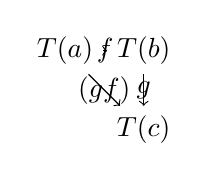
\begin{tikzpicture}
          \node (t a)                {$\funcO{T}(a)$};
          \node (t b) [right of=t a] {$\funcO{T}(b)$};
          \node (t c) [below of=t b] {$\funcO{T}(c)$};

          \draw [->] (t a) to node        {$\monM{}{f}$}                    (t b);
          \draw [->] (t a) to node [swap] {$\monM{}{(\monM{}{g} \comp f)}$} (t c);
          \draw [->] (t b) to node        {$\monM{}{g}$}                    (t c);
        \end{tikzpicture}
      \end{center}
      \caption{Kleisli triple associativity.}
      \label{fig:triple-associativity}
    \end{subfigure}
    \begin{subfigure}[b]{0.5\linewidth}
      \begin{center}
        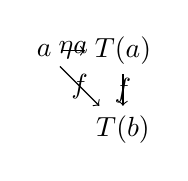
\begin{tikzpicture}
          \node (a)                  {$a$};
          \node (t a) [right of=a]   {$\funcO{T}(a)$};
          \node (t b) [below of=t a] {$\funcO{T}(b)$};

          \draw [->] (a)   to node        {$\natO{\eta}{a}$} (t a);
          \draw [->] (a)   to node [swap] {$f$}              (t b);
          \draw [->] (t a) to node        {$\monM{}{f}$}     (t b);
        \end{tikzpicture}
      \end{center}
      \caption{Kleisli triple unity.}
      \label{fig:triple-unity}
    \end{subfigure}
    \caption{}
  \end{figure}
\end{definition}

\begin{remark}
  \label{re:triple}

  Intuitively, \natO{\eta}{a} is the inclusion of values into
  computations and \monM{T}{f} is the extension of a function $f$ from
  values to computations to a function from computations to
  computations, which first evaluates a computation and then applies
  $f$ to the resulting value \parencite[59]{moggi-1991}.

\end{remark}

\begin{terminology}
  \label{ter:triple}

  The common term for Kleisli triples is Kleisli triple. Yet
  another term is algebraic theory in extension form
  \parencite[32]{manes-1976}, which is perhaps more precise but rather
  outdated. Despite the fact that the latter could be updated to
  something like monad in extension form, we choose
  Kleisli triple for the sake of simplicity. When defining
  monads, \textcite[138]{maclane-1998} considers the use of
  triple as ``frequent but unfortunate,'' but this is not the
  case within the context of this dissertation. \todo{Why or do not
    mention it.}

\end{terminology}

\begin{remark*}
  \label{re:monad-triple}

  Note that, contrary to the definition of a monad, a Kleisli triple does not
  require an endofunctor and its unit is not required to be defined as
  a natural transformation.

\end{remark*}

...

\begin{example}
  \label{ex:triple-identity}

  The most basic example of a Kleisli triple is the identity or
  trivial Kleisli triple, which is just a reformulation of the
  identity functor, just like Example \ref{ex:monad-identity}.

  Given a category \cat{C}, its identity function
  \eqref{eq:category-identity}, and the object and morphism functions
  of its identity endofunctor (Example \ref{ex:functor-identity})
  yield a Kleisli triple
  \begin{equation*}
    \mon{I} = (\funcO{I}, \id, \funcM{I})
    \text{,}
  \end{equation*}
  in \cat{C}, called the identity Kleisli triple.

  \begin{proof}

    Equation \eqref{eq:triple-associativity} holds by
    \eqref{eq:category-associativity}, and \eqref{eq:triple-unity-left}
    and \eqref{eq:triple-unity-right} hold by
    \eqref{eq:category-identity}.

  \end{proof}

\end{example}

\begin{examples}
  \label{ex:triple-notions-computation}

  %% \parencite[60]{moggi-1991}

  \hfill
  \begin{description}
  \item[Partiality]
  \item[Nondeterminism]
  \item[Side effects]
  \item[Exceptions]
  \item[Continuations]
  \item[Interactive input]
  \item[Interactive output]
  \end{description}
\end{examples}

\subsection*{Monads $=$ Kleisli triples}

Algebraic theories in clone form \parencite[24]{manes-1976}, which
will be referred to as monads in clone form, are yet another
alternative description for monads. \textcite[26--29]{manes-1976}
thoroughly proves the equivalence between monads and theories, and
leaves the proof of the equivalence between theories and Kleisli triples as an
exercise. \textcite[61]{moggi-1991} states the equivalence between
monads and Kleisli triples, but his proof does not contain details. The
following theorems demonstrate that monads and Kleisli triples are equivalent.
As illustrated in Figure \ref{fig:monad-theory-triple}, these proofs
are enough for stating the equivalence between the three alternative
descriptions.

\begin{figure}[htbp]
  \begin{center}
    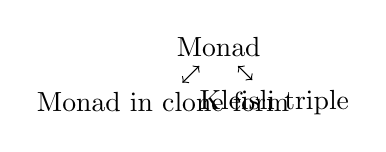
\begin{tikzpicture}
      \node (monad)                         {Monad};
      \node (theory) [below left of=monad]  {Monad in clone form};
      \node (triple) [below right of=monad] {Kleisli triple};

      \draw [<->] (monad) to (theory);
      \draw [<->] (monad) to (triple);
    \end{tikzpicture}
  \end{center}
  \caption{Monads $=$ Monads in clone form $=$ Kleisli triples.}
  \label{fig:monad-theory-triple}
\end{figure}

Lemma \ref{lem:monad-to-triple} states that a Kleisli triple can be obtained
from a monad. Note that, since monads are defined in terms of functors
and natural transformations, this lemma is simpler than its converse.

\begin{lemma}
  \label{lem:monad-to-triple}

  Let $\mon{T} = (\func{T}, \nat{\eta}, \nat{\mu})$ be a monad in a
  category \cat{C}. Then
  \begin{equation*}
    \mon{T} = (\funcO{T}, \nat{\eta}, \monM{}{\underscore})
    \text{,}
  \end{equation*}
  where \funcO{T} is the object function of the endofunctor \func{T},
  \nat{\eta} is the underlying transformation of the natural
  transformation \nat{\eta}, and $\monM{}{\underscore}: \catM{C} \to \catM{C}$
  is a morphism function which assigns to each morphism $f : a \to
  \funcO{T}(b) \in \catM{C}$ a morphism $\monM{}{f}: \funcO{T}(a) \to
  \funcO{T}(b) \in \catM{C}$ defined by\footnote{This definition is
    taken from \parencite[61]{moggi-1991}.}
  \begin{equation}
    \label{eq:monad-to-triple-extension}
    \monM{}{f} = \natO{\mu}{b} \comp \funcM{T}(f)
    \text{,}
  \end{equation}
  is a Kleisli triple in \cat{C}.

  \begin{proof}

    As
    \begin{steps}
      \stepm{\monM{}{\natO{\eta}{a}}}
        \eqbydef{$\monM{}{\natO{\eta}{a}}$ \eqref{eq:monad-to-triple-extension}}
      \stepm{\natO{\mu}{a} \comp \funcM{T}(\natO{\eta}{a})}
        \eqby{\eqref{eq:monad-unity-right}}
      \stepm{\idO{\funcO{T}(a)}},
    \end{steps}
    \eqref{eq:triple-unity-left} holds. Equation \eqref{eq:triple-unity-right}
    holds because
    \begin{steps}
      \stepm{\monM{}{f} \comp \natO{\eta}{a}}
        \eqbydef{$\monM{}{f}$ \eqref{eq:monad-to-triple-extension}}
      \stepm{\natO{\mu}{b} \comp \funcM{T}(f) \comp \natO{\eta}{a}}
        \eqby{\eqref{eq:monad-naturality-unit}}
      \stepm{\natO{\mu}{b} \comp \natO{\eta}{\funcO{T}(b)} \comp f}
        \eqby{\eqref{eq:monad-unity-left} with $a = b$}
      \stepm{\idO{\funcO{T}(b)} \comp f}
        \eqby{\eqref{eq:category-identity}}
      \stepm{f}.
    \end{steps}
    And, since
    \begin{steps}
      \stepm{\monM{}{g} \comp \monM{}{f}}
        \eqbydef{$\monM{}{f}$ and $\monM{}{g}$ \eqref{eq:monad-to-triple-extension}}
      \stepm{\natO{\mu}{c} \comp \funcM{T}(g) \comp \natO{\mu}{b} \comp \funcM{T}(f)}
        \eqby{\eqref{eq:monad-naturality-multiplication} with $f = g$}
      \stepm{\natO{\mu}{c} \comp \natO{\mu}{\funcO{T}(c)} \comp \funcM{T}(\funcM{T}(g)) \comp \funcM{T}(f)}
        \eqby{\eqref{eq:functor-composition} with $g = \funcM{T}(g)$}
      \stepm{\natO{\mu}{c} \comp \natO{\mu}{\funcO{T}(c)} \comp \funcM{T}(\funcM{T}(g) \comp f)}
        \eqby{\eqref{eq:monad-associativity} with $a = c$}
      \stepm{\natO{\mu}{c} \comp \funcM{T}(\natO{\mu}{c}) \comp \funcM{T}(\funcM{T}(g) \comp f)}
        \eqby{\eqref{eq:functor-composition} with $f = \funcM{T}(g) \comp f$ and $g = \natO{\mu}{c}$}
      \stepm{\natO{\mu}{c} \comp \funcM{T}(\natO{\mu}{c} \comp \funcM{T}(g) \comp f)}
        \eqbydef{$\monM{}{g}$ and \monM{}{(\monM{}{g} \comp f)} \eqref{eq:monad-to-triple-extension}}
      \stepm{\monM{}{(\monM{}{g} \comp f)}},
    \end{steps}
    \eqref{eq:triple-associativity} holds.

  \end{proof}

\end{lemma}

The object function of a Kleisli triple can be extended to define an
endofunctor. Lemma \ref{prop:triple-to-endofunctor} states that
an endofunctor can be derived from a Kleisli triple.

\begin{proposition}
  \label{prop:triple-to-endofunctor}

  If $\mon{T} = (\funcO{T}, \nat{\eta}, \monM{}{\underscore})$ is a Kleisli triple in
  a category \cat{C}, then
  \begin{equation*}
    \func{T} = (\funcO{T}, \funcM{T})
    \text{,}
  \end{equation*}
  where $\funcM{T}: \catM{C} \to \catM{C}$ is a morphism function
  which assigns to each morphism $f: a \to b \in \catM{C}$ a morphism
  $\funcM{T}(f): \funcO{T}(a) \to \funcO{T}(b) \in \catM{C}$ defined
  by\footnote{This definition is taken from
    \parencite[61]{moggi-1991}.}
  \begin{equation}
    \label{eq:triple-to-endofunctor-morphism-function}
    \funcM{T}(f) = \monM{}{(\natO{\eta}{b} \comp f)}
    \text{,}
  \end{equation}
  is an endofunctor in \cat{C}.

  \begin{proof}

    Equation \eqref{eq:functor-identity} holds because
    \begin{steps}
      \stepm{\funcM{T}(\idO{a})}
        \eqbydef{$\funcM{T}(\idO{a})$ \eqref{eq:triple-to-endofunctor-morphism-function}}
      \stepm{\monM{}{(\natO{\eta}{a} \comp \idO{a})}}
        \eqby{\eqref{eq:category-identity} with $f = \natO{\eta}{a}$}
      \stepm{\monM{}{\natO{\eta}{a}}}.
    \end{steps}
    And \eqref{eq:functor-composition} holds because
    \begin{steps}
      \stepm{\funcM{T}(g \comp f)}
        \eqbydef{$\funcM{T}(g \comp f)$ \eqref{eq:triple-to-endofunctor-morphism-function}}
      \stepm{\monM{}{(\natO{\eta}{c} \comp g \comp f)}}
        \eqby{\eqref{eq:triple-unity-left} with $f = \natO{\eta}{c} \comp g$}
      \stepm{\monM{}{(\monM{}{(\natO{\eta}{c} \comp g)} \comp \natO{\eta}{b} \comp f)}}
        \eqby{\eqref{eq:triple-associativity} with $f = \natO{\eta}{b} \comp f$ and $g = \natO{\eta}{c} \comp g$}
      \stepm{\monM{}{(\natO{\eta}{c} \comp g)} \comp \monM{}{(\natO{\eta}{b} \comp f)}}
        \eqbydef{$\funcM{T}(f)$ and $\funcM{T}(g)$ \eqref{eq:triple-to-endofunctor-morphism-function}}
      \stepm{\funcM{T}(g) \comp \funcM{T}(f)}.
    \end{steps}

  \end{proof}

\end{proposition}

Since \func{T} is an endofunctor, it is now possible to ask if
\nat{\eta} is a natural transformation. Lemma
\ref{prop:triple-to-monad-unit} states and proves that it is.

\begin{proposition}
  \label{prop:triple-to-monad-unit}

  If $\mon{T} = (\funcO{T}, \nat{\eta}, \monM{}{\underscore})$ is a Kleisli triple in
  a category \cat{C}, then the transformation \nat{\eta} is natural.

  \begin{proof}

    As
    \begin{steps}
      \stepm{\natO{\eta}{\funcO{T}(b)} \comp f}
        \eqby{\eqref{eq:triple-unity-left} with $f = \natO{\eta}{\funcO{T}(b)} \comp f$}
      \stepm{\monM{}{(\natO{\eta}{\funcO{T}(b)} \comp f)} \comp \natO{\eta}{a}}
        \eqbydef{$\funcM{T}(f)$ \eqref{eq:triple-to-endofunctor-morphism-function}}
      \stepm{\funcM{T}(f) \comp \natO{\eta}{a}},
    \end{steps}
    \nat{\eta} is natural.

  \end{proof}

\end{proposition}

Lemma \ref{prop:triple-to-monad-multiplication} defines the
multiplication function of a monad given a Kleisli triple, and proves that it
is a natural transformation.

\begin{proposition}
  \label{prop:triple-to-monad-multiplication}

  If $\mon{T} = (\funcO{T}, \nat{\eta}, \monM{}{\underscore})$ is a Kleisli triple in
  a category \cat{C}, then a function $\nat{\mu}: \catO{C} \to
  \catM{C}$ which assigns to each object $a \in \catO{C}$ a morphism
  $\natO{\mu}{a}: \funcO{T}(\funcO{T}(a)) \to \funcO{T}(a) \in
  \catM{C}$ defined by\footnote{This definition is taken from
    \parencite[61]{moggi-1991}.}
  \begin{equation}
    \label{eq:triple-to-monad-multiplication}
    \natO{\mu}{a} = \monM{}{\idO{\funcO{T}(a)}}
  \end{equation}
  is a natural transformation $\nat{\mu}: \func{T} \comp \func{T} \to
  \func{T}: \cat{C} \to \cat{C}$.

  \begin{proof}

    Since
    \begin{steps}
      \stepm{\natO{\mu}{\funcO{T}(b)} \comp \funcM{T}(\funcM{T}(f))}
        \eqbydef{$\natO{\mu}{\funcO{T}(b)}$ \eqref{eq:triple-to-monad-multiplication}}
      \stepm{\monM{}{\idO{\funcO{T}(\funcO{T}(b))}} \comp \funcM{T}(\funcM{T}(f))}
        \eqbydef{$\funcM{T}(f)$ \eqref{eq:triple-to-endofunctor-morphism-function}}
      \stepm{\monM{}{\idO{\funcO{T}(\funcO{T}(b))}} \comp \funcM{T}(\monM{}{(\natO{\eta}{\funcO{T}(b)} \comp f)})}
        \eqbydef{$\funcM{T}(\monM{}{(\natO{\eta}{\funcO{T}(b)} \comp f)})$ \eqref{eq:triple-to-endofunctor-morphism-function}}
      \stepm{\monM{}{\idO{\funcO{T}(\funcO{T}(b))}} \comp \monM{}{(\natO{\eta}{\funcO{T}(\funcO{T}(b))} \comp \monM{}{(\natO{\eta}{\funcO{T}(b)} \comp f)})}}
        \eqby{\eqref{eq:triple-associativity} with $f = \natO{\eta}{\funcO{T}(\funcO{T}(b))} \comp \monM{}{(\natO{\eta}{\funcO{T}(b)} \comp f)}$ and $g = \idO{\funcO{T}(\funcO{T}(b))}$}
      \stepm{\monM{}{(\monM{}{\idO{\funcO{T}(\funcO{T}(b))}} \comp \natO{\eta}{\funcO{T}(\funcO{T}(b))} \comp \monM{}{(\natO{\eta}{\funcO{T}(b)} \comp f)})}}
        \eqby{\eqref{eq:triple-unity-left} with $f = \idO{\funcO{T}(\funcO{T}(b))}$}
      \stepm{\monM{}{(\idO{\funcO{T}(\funcO{T}(b))} \comp \monM{}{(\natO{\eta}{\funcO{T}(b)} \comp f)})}}
        \eqby{\eqref{eq:category-identity} with $f = \monM{}{(\natO{\eta}{\funcO{T}(b)} \comp f)}$}
      \stepm{\monM{}{(\monM{}{(\natO{\eta}{\funcO{T}(b)} \comp f)})}}
        \eqby{\eqref{eq:category-identity} with $f = \monM{}{(\natO{\eta}{\funcO{T}(b)} \comp f)}$}
      \stepm{\monM{}{(\monM{}{(\natO{\eta}{\funcO{T}(b)} \comp f)} \comp \idO{\funcO{T}(a)})}}
        \eqby{\eqref{eq:triple-associativity} with $f = \idO{\funcO{T}(a)}$ and $g = \natO{\eta}{\funcO{T}(b)} \comp f$}
      \stepm{\monM{}{(\natO{\eta}{\funcO{T}(b)} \comp f)} \comp \monM{}{\idO{\funcO{T}(a)}}}
        \eqbydef{$\funcM{T}(f)$ \eqref{eq:triple-to-endofunctor-morphism-function}}
      \stepm{\funcM{T}(f) \comp \monM{}{\idO{\funcO{T}(a)}}}
        \eqbydef{$\natO{\mu}{a}$ \eqref{eq:triple-to-monad-multiplication}}
      \stepm{\funcM{T}(f) \comp \natO{\mu}{a}},
    \end{steps}
    then \nat{\mu} is natural.

  \end{proof}

\end{proposition}

Lemma \ref{lem:triple-to-monad} states that a monad can be obtained
from a Kleisli triple using the constructions from the three propositions
above.

\begin{lemma}
  \label{lem:triple-to-monad}

  Let $\mon{T} = (\funcO{T}, \nat{\eta}, \monM{}{\underscore})$ be a Kleisli triple in
  a category \cat{C}. Then
  \begin{equation*}
    \mon{T} = (\func{T}, \nat{\eta}, \nat{\mu})
    \text{,}
  \end{equation*}
  where \func{T} is the endofunctor in \cat{C} defined by Lemma
  \ref{prop:triple-to-endofunctor}, \nat{\eta} is the transformation
  \nat{\eta} regarded as a natural transformation (see Lemma
  \ref{prop:triple-to-monad-unit}), and $\nat{\mu}: \func{T} \comp
  \func{T} \to \func{T}: \cat{C} \to \cat{C}$ is the natural
  transformation defined by Lemma
  \ref{prop:triple-to-monad-multiplication}, is a monad in \cat{C}.

  \begin{proof}

    As
    \begin{steps}
      \stepm{\natO{\mu}{a} \comp \natO{\mu}{\funcO{T}(a)}}
        \eqbydef{$\natO{\mu}{a}$ and $\natO{\mu}{\funcO{T}(a)}$ \eqref{eq:triple-to-monad-multiplication}}
      \stepm{\monM{}{\idO{\funcO{T}(a)}} \comp \monM{}{\idO{\funcO{T}(\funcO{T}(a))}}}
        \eqby{\eqref{eq:triple-associativity} with $f = \idO{\funcO{T}(\funcO{T}(a))}$ and $g = \idO{\funcO{T}(a)}$}
      \stepm{\monM{}{(\monM{}{\idO{\funcO{T}(a)}} \comp \idO{\funcO{T}(\funcO{T}(a))})}}
        \eqby{\eqref{eq:category-identity} with $f = \monM{}{\idO{\funcO{T}(a)}}$}
      \stepm{\monM{}{(\monM{}{\idO{\funcO{T}(a)}})}}
        \eqby{\eqref{eq:category-identity} with $f = \monM{}{\idO{\funcO{T}(a)}}$}
      \stepm{\monM{}{(\idO{\funcO{T}(a)} \comp \monM{}{\idO{\funcO{T}(a)}})}}
        \eqby{\eqref{eq:triple-unity-left} with $f = \idO{\funcO{T}(a)}$}
      \stepm{\monM{}{(\monM{}{\idO{\funcO{T}(a)}} \comp \natO{\eta}{\funcO{T}(a)} \comp \monM{}{\idO{\funcO{T}(a)}})}}
        \eqby{\eqref{eq:triple-associativity} with $f = \natO{\eta}{\funcO{T}(a)} \comp \monM{}{\idO{\funcO{T}(a)}}$ and $g = \idO{\funcO{T}(a)}$}
      \stepm{\monM{}{\idO{\funcO{T}(a)}} \comp \monM{}{(\natO{\eta}{\funcO{T}(a)} \comp \monM{}{\idO{\funcO{T}(a)}})}}
        \eqbydef{$\natO{\mu}{a}$ \eqref{eq:triple-to-monad-multiplication}}
      \stepm{\natO{\mu}{a} \comp \monM{}{(\natO{\eta}{\funcO{T}(a)} \comp \natO{\mu}{a})}}
        \eqbydef{$\funcM{T}(\natO{\mu}{a})$ \eqref{eq:triple-to-endofunctor-morphism-function}}
      \stepm{\natO{\mu}{a} \comp \funcM{T}(\natO{\mu}{a})},
    \end{steps}
    \eqref{eq:monad-associativity} holds. And, since
    \begin{steps}
      \stepm{\natO{\mu}{a} \comp \natO{\eta}{\funcO{T}(a)}}
        \eqbydef{$\natO{\mu}{a}$ \eqref{eq:triple-to-monad-multiplication}}
      \stepm{\monM{}{\idO{\funcO{T}(a)}} \comp \natO{\eta}{\funcO{T}(a)}}
        \eqby{\eqref{eq:triple-unity-left} with $f = \idO{\funcO{T}(a)}$}
      \stepm{\idO{\funcO{T}(a)}}
    \end{steps}
    and
    \begin{steps}
      \stepm{\natO{\mu}{a} \comp \funcM{T}(\natO{\eta}{a})}
        \eqbydef{$\natO{\mu}{a}$ \eqref{eq:triple-to-monad-multiplication}}
      \stepm{\monM{}{\idO{\funcO{T}(a)}} \comp \funcM{T}(\natO{\eta}{a})}
        \eqbydef{$\funcM{T}(\natO{\eta}{a})$ \eqref{eq:triple-to-endofunctor-morphism-function}}
      \stepm{\monM{}{\idO{\funcO{T}(a)}} \comp \monM{}{(\natO{\eta}{\funcO{T}(a)} \comp \natO{\eta}{a})}}
        \eqby{\eqref{eq:triple-associativity} with $f = \natO{\eta}{\funcO{T}(a)} \comp \natO{\eta}{a}$ and $g = \idO{\funcO{T}(a)}$}
      \stepm{\monM{}{(\monM{}{\idO{\funcO{T}(a)}} \comp \natO{\eta}{\funcO{T}(a)} \comp \natO{\eta}{a})}}
        \eqby{\eqref{eq:triple-unity-left} with $f = \idO{\funcO{T}(a)}$}
      \stepm{\monM{}{(\idO{\funcO{T}(a)} \comp \natO{\eta}{a})}}
        \eqby{\eqref{eq:category-identity} with $f = \natO{\eta}{a}$}
      \stepm{\monM{}{\natO{\eta}{a}}}
        \eqby{\eqref{eq:triple-unity-right}}
      \stepm{\idO{\funcO{T}(a)}},
    \end{steps}
    then \eqref{eq:monad-unity-left} and \eqref{eq:monad-unity-right}
    hold.

  \end{proof}

\end{lemma}

Finally, Theorem \ref{the:monad-triple} proves that monads and Kleisli triples
are equivalent.

\begin{theorem}
  \label{the:monad-triple}

  Monads and Kleisli triples are coextensive.

  \begin{proof}

    The correspondence between monads and Kleisli triples is given by Lemma
    \ref{lem:monad-to-triple}, which proves that a Kleisli triple can be
    derived from a monad, and Lemma \ref{lem:triple-to-monad}, which proves
    that a monad can be derived from a Kleisli triple.

  \end{proof}

\end{theorem}

\begin{example}
  \label{ex:monad-triple-identity}

\end{example}

\todo{These theorems will be mentioned in Section \ref{sec:monads-agda}.}

\section{Monads in Haskell}
\label{sec:monads-haskell}

When discussing monads, there are three possibilities, as previously
mentioned: monads (in monoid form), monads in extension form (Kleisli
triples), and monads in clone form. Since monads in extension form are
easier to justify from a computational point of view, this
representation is the one found in functional programming languages
like Haskell. We study monads (in monoid form) first and then Kleisli
triples. Note, however, that studying only Kleisli triples would be
enough, but monads have some mathematical advantages and are more
intuitive in some cases. Finally, studying monads in clone form would
also imply some mathematical advantages (just like the monadic laws
are very similar to the laws of a monoid, the monadic laws in clone
form are very similar to the laws of a category).

\subsection*{Monads}

A monad in \hask consists of an endofunctor \texttt{m}, which
corresponds to \eqref{eq:monad-}, together with two parametrically
polymorphic functions
\begin{equation}
  \label{eq:monad-return-haskell}
  \text{\texthaskell{return :: a -> m a}}
\end{equation}
and
\begin{equation}
  \label{eq:monad-join-haskell}
  \text{\texthaskell{join :: m (m a) -> m a}}
  \text{,}
\end{equation}
which correspond to \eqref{eq:monad-unit} and
\eqref{eq:monad-multiplication}, respectively, in such a way that, for
all types \texthaskell{a} $\in \catO{\hask}$, the diagrams in Figures
\ref{fig:monad-associativity-haskell} and
\ref{fig:monad-unity-haskell} are commutative, or, equivalently,
\begin{equation}
  \label{eq:monad-associativity-haskell}
  \text{\texthaskell{join . join = join . fmap join}}
  \text{,}
\end{equation}
\begin{equation}
  \label{eq:monad-unity-left-haskell}
  \text{\texthaskell{join . return = id}}
  \text{,}
\end{equation}
and
\begin{equation}
  \label{eq:monad-unity-right-haskell}
  \text{\texthaskell{join . fmap return = id}}
  \text{,}
\end{equation}
which correspond to \eqref{eq:monad-associativity},
\eqref{eq:monad-unity-left}, and \eqref{eq:monad-unity-right},
respectively.
\begin{figure}[htb]
  \begin{center}
    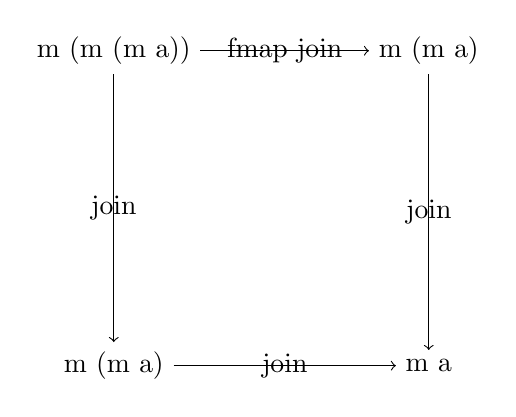
\begin{tikzpicture}[node distance=4cm]
      \node (ttt a)                  {\texthaskell{m (m (m a))}};
      \node (tt a1) [right of=ttt a] {\texthaskell{m (m a)}};
      \node (tt a2) [below of=ttt a] {\texthaskell{m (m a)}};
      \node (t a)   [right of=tt a2] {\texthaskell{m a}};

      \draw [->] (ttt a) to node        {\texthaskell{fmap join}} (tt a1);
      \draw [->] (ttt a) to node [swap] {\texthaskell{join}}      (tt a2);
      \draw [->] (tt a1) to node        {\texthaskell{join}}      (t a);
      \draw [->] (tt a2) to node [swap] {\texthaskell{join}}      (t a);
    \end{tikzpicture}
  \end{center}
  \caption{Monadic associativity in \hask.}
  \label{fig:monad-associativity-haskell}
\end{figure}
\begin{figure}[htb]
  \begin{center}
    \begin{tikzpicture}[node distance=4cm]
      \node (it a)                 {\texthaskell{m a}};
      \node (tt a) [right of=it a] {\texthaskell{m (m a)}};
      \node (ti a) [right of=tt a] {\texthaskell{m a}};
      \node (t a2) [right of=t a1] {\texthaskell{m a}};


      \draw [->] (it a) to node        {\texthaskell{return}}      (tt a);
      \draw [->] (ti a) to node [swap] {\texthaskell{fmap return}} (tt a);

      \draw [->]     (tt a) to node {\texthaskell{join}} (t a2);

      \draw [->] (it a) to node [swap] {\texthaskell{id}} (t a2);
      \draw [->] (ti a) to node        {\texthaskell{id}} (t a2);
    \end{tikzpicture}
  \end{center}
  \caption{Monadic unity in \hask.}
  \label{fig:monad-unity-haskell}
\end{figure}

Additionally, since \texthaskell{return}
\eqref{eq:monad-return-haskell} and \texthaskell{join}
\eqref{eq:monad-join-haskell} are parametrically polymorphic
functions, then, by parametricity (see Section
\ref{sec:naturals-haskell}), for all functions
\begin{equation*}
  \text{\texthaskell{f :: a -> m b}} \in \catM{\hask}
  \text{,}
\end{equation*}
\begin{equation}
  \label{eq:monad-naturality-return-haskell}
  \text{\texthaskell{return . f = fmap f . return}}
\end{equation}
and
\begin{equation}
  \label{eq:monad-naturality-join-haskell}
  \text{\texthaskell{join . fmap (fmap f) = fmap f . join}}
  \text{,}
\end{equation}
which correspond to \eqref{eq:monad-naturality-unit} and
\eqref{eq:monad-naturality-multiplication}, respectively.

Monads in \hask are defined by the \texthaskell{Monad'} type class,
whose declaration appears in Figure \ref{fig:monad-haskell} and which is not a standard type class. As usual,
notice that monadic associativity and unity, that is,
\eqref{eq:monad-associativity-haskell},
\eqref{eq:monad-unity-left-haskell}, and
\eqref{eq:monad-unity-right-haskell}, and monadic naturalities, that
is, \eqref{eq:monad-naturality-return-haskell} and
\eqref{eq:monad-naturality-join-haskell}, are not part of this
declaration. As mentioned earlier, however, the latter need not be
part of it because they are free theorems.
\begin{figure}[htbp]
  \begin{codehaskell}
class Functor m => Monad' m where
  return :: a -> m a
  join   :: m (m a) -> m a
  \end{codehaskell}
  \caption{The \texthaskell{Monad'} type class.}
  \label{fig:monad-haskell}
\end{figure}

\todo{Surprise, surprise, where is \hask's identity functor?}

\begin{example}
  \label{ex:monad-identity-haskell}

  Unlike Examples \ref{ex:monad-identity} and
  \ref{ex:triple-identity}, the identity monad in \hask is an
  intuitive way of learning to use the \texthaskell{Monad'} type
  class. It is just a redefinition of the identity functor, but its
  instance declaration, which appears in Figure
  \ref{fig:monad-identity-haskell}, gives a good idea of what
  \texthaskell{return} and \texthaskell{join} do.

  \begin{figure}[htbp]
    \begin{codehaskell}
instance Monad' Identity where
  return = Identity

  join (Identity mx) = mx
    \end{codehaskell}
    \caption{The \texthaskell{Identity} \texthaskell{Monad'}.}
    \label{fig:monad-identity-haskell}
  \end{figure}

  \begin{proof}

    ...

  \end{proof}

\end{example}

\begin{example}
  \label{ex:monad-maybe-haskell}

  The \texthaskell{Maybe} monad in \hask consists of the
  \texthaskell{Maybe} endofunctor (Example
  \ref{ex:functor-maybe-haskell}), a unit function
  \begin{equation*}
    \text{\texthaskell{return :: a -> Maybe a}}
    \text{,}
  \end{equation*}
  defined by
  \begin{equation}
    \label{eq:maybe-return}
    \text{\texthaskell{return = Just}}
    \text{,}
  \end{equation}
  and a multiplication function
  \begin{equation*}
    \text{\texthaskell{join :: Maybe (Maybe a) -> Maybe a}}
    \text{,}
  \end{equation*}
  defined by
  \begin{equation}
    \label{eq:maybe-join-nothing}
    \text{\texthaskell{join Nothing = Nothing}}
  \end{equation}
  and
  \begin{equation}
    \label{eq:maybe-join-just}
    \text{\texthaskell{join (Just mx) = mx}}
    \text{.}
  \end{equation}

  The \texthaskell{Monad'} instance declaration for the
  \texthaskell{Maybe} type is shown in Figure
  \ref{fig:monad-maybe-haskell}.
  \begin{figure}[htbp]
    \begin{codehaskell}
instance Monad' Maybe where
  return = Just

  join Nothing   = Nothing
  join (Just mx) = mx
    \end{codehaskell}
    \caption{The \texthaskell{Maybe} monad in \hask.}
    \label{fig:monad-maybe-haskell}
  \end{figure}

  \begin{proof}

    Equation \eqref{eq:monad-associativity-haskell} holds because
    \begin{steps}
      \steph{(join . join) Nothing}
        \eqbydef{\texthaskell{(.)}}
      \steph{join (join Nothing)}
        \eqbydef{\texthaskell{join} \eqref{eq:maybe-join-nothing}}
      \steph{join Nothing}
        \eqbydef{\texthaskell{fmap}}
      \steph{join (fmap join Nothing)}
        \eqbydef{\texthaskell{(.)}}
      \steph{(join . fmap join) Nothing}
    \end{steps}
    and
    \begin{steps}
      \steph{(join . join) (Just mmx)}
        \eqbydef{\texthaskell{(.)}}
      \steph{join (join (Just mmx))}
        \eqbydef{\texthaskell{join} \eqref{eq:maybe-join-just}}
      \steph{join mmx}
        \eqbydef{\texthaskell{join} \eqref{eq:maybe-join-just}}
      \steph{join (Just (join mmx))}
        \eqbydef{\texthaskell{fmap}}
      \steph{join (fmap join (Just mmx))}
        \eqbydef{\texthaskell{(.)}}
      \steph{(join . fmap join) (Just mmx)}.
    \end{steps}
    As
    \begin{steps}
      \steph{(join . return) mx}
        \eqbydef{\texthaskell{(.)}}
      \steph{join (return mx)}
        \eqbydef{\texthaskell{return} \eqref{eq:maybe-return}}
      \steph{join (Just mx)}
        \eqbydef{\texthaskell{join} \eqref{eq:maybe-join-just}}
      \steph{mx}
        \eqbydef{\texthaskell{id}}
      \steph{id mx},
    \end{steps}
    \eqref{eq:monad-unity-left} holds. And, since
    \begin{steps}
      \steph{(join . fmap return) Nothing}
        \eqbydef{\texthaskell{(.)}}
      \steph{join (fmap return Nothing)}
        \eqbydef{\texthaskell{fmap}}
      \steph{join Nothing}
        \eqbydef{\texthaskell{join} \eqref{eq:maybe-join-nothing}}
      \steph{Nothing}
        \eqbydef{\texthaskell{id}}
      \steph{id Nothing}
    \end{steps}
    and
    \begin{steps}
      \steph{(join . fmap return) (Just x)}
        \eqbydef{\texthaskell{(.)}}
      \steph{join (fmap return (Just x))}
        \eqbydef{\texthaskell{fmap}}
      \steph{join (Just (return x))}
        \eqbydef{\texthaskell{join} \eqref{eq:maybe-join-just}}
      \steph{return x}
        \eqbydef{\texthaskell{return} \eqref{eq:maybe-return}}
      \steph{Just x}
        \eqbydef{\texthaskell{id}}
      \steph{id (Just x)},
    \end{steps}
    then \eqref{eq:monad-unity-right-haskell} holds.

  \end{proof}

\end{example}

\begin{example}
  \label{ex:monad-list-haskell}

  The list monad in \hask consists of the list endofunctor (Example
  \ref{ex:functor-list-haskell}, a unit function
  \begin{equation*}
    \text{\texthaskell{return :: a -> [a]}}
  \end{equation*}
  defined by
  \begin{equation}
    \label{eq:list-return}
    \text{\texthaskell{return x = [x]}}
    \text{,}
  \end{equation}
  and a multiplication function
  \begin{equation*}
    \text{\texthaskell{join :: [[a]] -> [a]}}
  \end{equation*}
  defined by
  \begin{equation}
    \label{eq:list-join}
    \text{\texthaskell{join = concat}}
    \text{,}
  \end{equation}
  where
  \begin{equation*}
    \text{\texthaskell{concat :: [[a]] -> [a]}}
  \end{equation*}
  is given by
  \begin{equation}
    \label{eq:list-concat-nil}
    \text{\texthaskell{concat [] = []}}
  \end{equation}
  and
  \begin{equation}
    \label{eq:list-concat-cons}
    \text{\texthaskell{concat (xs:xss) = xs ++ concat xss}}
    \text{,}
  \end{equation}
  and
  \begin{equation*}
    \text{\texthaskell{(++) :: [a] -> [a] -> [a]}}
  \end{equation*}
  is given by
  \begin{equation}
    \text{\texthaskell{[] ++ ys = ys}}
  \end{equation}
  and
  \begin{equation}
    \text{\texthaskell{(x:xs) ++ ys = x : xs ++ ys}}
    \text{.}
  \end{equation}

  Figure \ref{fig:monad-list-haskell} presents the instance
  declaration for lists.
  \begin{figure}[htbp]
    \begin{codehaskell}
instance Monad' [] where
  return x = [x]

  join = concat
    \end{codehaskell}
    \caption{The \texthaskell{[]} monad.}
    \label{fig:monad-list-haskell}
  \end{figure}

  \begin{proof}

    \hfill

    \begin{steps}
      \steph{join (join xsss)}

      \steph{join (fmap join xsss)}
    \end{steps}

    \begin{steps}
      \steph{(join . return) xs}

      \steph{join (return xs)}

      \steph{concat [xs]}

      \steph{concat (xs:[])}

      \steph{xs ++ concat []}

      \steph{xs ++ []}

      \steph{xs}

      \steph{id xs}
    \end{steps}

    \begin{steps}
      \steph{(join . fmap return) []}

      \steph{join (fmap return [])}

      \steph{concat []}

      \steph{[]}

      \steph{id []}
    \end{steps}

    \begin{steps}
      \steph{(join . fmap return) (x:xs)}

      \steph{join (fmap return (x:xs))}

      \steph{concat (return x : fmap return xs}

      \steph{return x ++ concat (fmap return xs)}

      \steph{return x ++ xs}

      \steph{x:xs}
    \end{steps}

  \end{proof}

\end{example}

\subsection*{Kleisli triples}

\todo{\texthaskell{bind} is actually \texthaskell{=<<}.}

Similary, a Kleisli triple in \hask consists of a type constructor
\texthaskell{m}, which corresponds to \eqref{eq:triple-}, a
parametrically polymorphic function \texthaskell{return}
\eqref{eq:monad-return-haskell}, which corresponds to
\eqref{eq:monad-unit}, and a function
\begin{equation}
  \label{eq:triple-alternative-bind-haskell}
  \text{\texthaskell{(>>=) :: m a -> (a -> m b) -> m b}}
  \text{,}
\end{equation}
or, better,
\begin{equation}
  \label{eq:triple-bind-haskell}
  \text{\texthaskell{bind :: (a -> m b) -> m a -> m b}}
  \text{,}
\end{equation}
which corresponds to \eqref{eq:triple-extension}, such that, for all
functions
\begin{equation*}
  \text{\texthaskell{f :: a -> m b}} \in \catM{\hask}
  \quad
  \text{and}
  \quad
  \text{\texthaskell{g :: b -> m c}} \in \catM{\hask}
  \text{,}
\end{equation*}
\begin{equation}
  \label{eq:triple-associativity-haskell}
  \text{\texthaskell{bind g . bind f = bind (bind g . f)}}
  \text{,}
\end{equation}
for all functions \texthaskell{f :: a -> m b} $\in \catM{\hask}$,
\begin{equation}
  \label{eq:triple-unity-left-haskell}
  \text{\texthaskell{bind f . return = f}}
  \text{,}
\end{equation}
and
\begin{equation}
  \label{eq:triple-unity-right-haskell}
  \text{\texthaskell{bind return = id}}
  \text{,}
\end{equation}
which correspond to \eqref{eq:triple-associativity},
\eqref{eq:triple-unity-left}, and \eqref{eq:triple-unity-right},
respectively, or, equivalently, such that the diagrams in Figures
\ref{fig:triple-associativity-haskell} and
\ref{fig:triple-unity-haskell} are commutative, and
\eqref{eq:triple-unity-right-haskell}.
\begin{figure}[htb]
  \begin{subfigure}[b]{0.5\linewidth}
    \begin{center}
      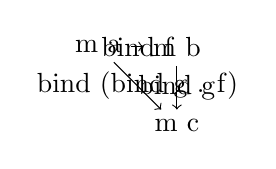
\begin{tikzpicture}
        \node (t a)                {\texthaskell{m a}};
        \node (t b) [right of=t a] {\texthaskell{m b}};
        \node (t c) [below of=t b] {\texthaskell{m c}};

        \draw [->] (t a) to node        {\texthaskell{bind f}}            (t b);
        \draw [->] (t a) to node [swap] {\texthaskell{bind (bind g . f)}} (t c);
        \draw [->] (t b) to node        {\texthaskell{bind g}}            (t c);
      \end{tikzpicture}
    \end{center}
    \caption{Monadic associativity.}
    \label{fig:triple-associativity-haskell}
  \end{subfigure}
  \begin{subfigure}[b]{0.5\linewidth}
    \begin{center}
      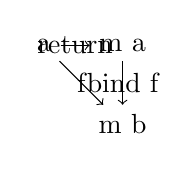
\begin{tikzpicture}
        \node (a)                  {\texthaskell{a}};
        \node (t a) [right of=a]   {\texthaskell{m a}};
        \node (t b) [below of=t a] {\texthaskell{m b}};

        \draw [->] (a)   to node        {\texthaskell{return}} (t a);
        \draw [->] (a)   to node [swap] {\texthaskell{f}}      (t b);
        \draw [->] (t a) to node        {\texthaskell{bind f}} (t b);
      \end{tikzpicture}
    \end{center}
    \caption{Monadic unity.}
    \label{fig:triple-unity-haskell}
  \end{subfigure}
  \caption{}
\end{figure}

Section \ref{sec:functors-haskell} details the correspondence between
an object function such as \eqref{eq:triple-} and a type constructor.
An important, and inevitable, difference between Definition
\ref{def:triple} and Kleisli triples in Haskell is that the former would not
require \texthaskell{return} to be a natural transformation, but it is
(by parametricity, all parametrically polymorphic functions are
natural transformations). Finally, the type signature of the
\texthaskell{bind} function could be rewritten as
\begin{equation*}
  \text{\texthaskell{bind :: (a -> m b) -> (m a -> m b)}}
  \text{,}
\end{equation*}
which makes it clear that it assigns a function to another function.

\todo{Specify the correspondence with the standard type class.}

Kleisli triples in \hask are defined by the \texthaskell{Monad} type class,
which corresponds to the minimal definition of the standard
\texthaskell{Monad} type class and whose declaration appears in Figure
\ref{fig:triple-haskell}. Notice that, as usual, this declaration does
not include \eqref{eq:triple-associativity-haskell},
\eqref{eq:triple-unity-left-haskell}, and
\eqref{eq:triple-unity-right-haskell}.
\begin{figure}[htbp]
  \begin{codehaskell}
class Monad m where
  return :: a -> m a
  bind   :: (a -> m b) -> m a -> m b
  \end{codehaskell}
  \caption{The \texthaskell{Monad} type class.}
  \label{fig:triple-haskell}
\end{figure}

The standard \texthaskell{Monad} type class is defined in terms of
\texthaskell{(>>=)}, as in Figure \ref{fig:standard-triple-haskell}.
Note that only the minimal definition is presented, that is,
\texthaskell{(>>)} and \texthaskell{fail} are not included. This
declaration is equivalent to that of Figure \ref{fig:triple-haskell},
but the latter is more suitable for abstract manipulation and for
comparing monads with Kleisli triples.

\begin{figure}[htbp]
  \begin{codehaskell}
class Monad m where
  return :: a -> m a
  (>>=)  :: m a -> (a -> m b) -> m b
  \end{codehaskell}
  \caption{The standard \texthaskell{Monad} type class.}
  \label{fig:standard-triple-haskell}
\end{figure}

\begin{remark}
  \label{re:triple-endofunctor}
  Note that not including a \texthaskell{Functor} type constraint to
  the \texthaskell{Triple} type class is actually more theoretically
  correct. However, since Lemma \ref{prop:triple-to-endofunctor}
  states that Kleisli triples are endofunctors, this type constraint could be
  included for practical reasons.

  For instance, it is preferable to use \texthaskell{fmap} instead of
  \texthaskell{liftM}. -- Find a better argument or ignore this.

\end{remark}

\begin{equation*}
  \text{\texthaskell{(>>=) :: Monad m => m a -> (a -> m b) -> m b}}
\end{equation*}
\begin{equation}
  \label{eq:triple-to-alternative-bind-haskell}
  \text{\texthaskell{mx >>= f = bind f mx}}
\end{equation}


Since
\begin{steps}
  \steph{(bind g . bind f) mx}
    \eqbydefh{(.)}
  \steph{bind g (bind f mx)}
    \eqbydefh{bind}
  \steph{(bind f mx) >>= g}
    \eqbydefh{bind}
  \steph{(mx >>= f) >>= g}
\end{steps}
and
\begin{steps}
  \steph{bind (bind g . f) mx}
    \eqbydefh{bind}
  \steph{mx >>= (bind g . f)}
    \eqbydefh{(.)}
  \steph{mx >>= (\textbackslash x -> bind g (f x))}
    \eqbydefh{bind}
  \steph{mx >>= (\textbackslash x -> f x >>= g)},
\end{steps}
\begin{steps}
  \steph{(bind f . return) x}
    \eqbydefh{(.)}
  \steph{bind f (return x)}
    \eqbydefh{bind}
  \steph{return x >>= f},
\end{steps}
and
\begin{steps}
  \steph{bind return mx}
    \eqbydef{\texthaskell{(>>=)} \eqref{eq:triple-to-alternative-bind-haskell}}
  \steph{mx >>= return},
\end{steps}
\eqref{eq:triple-unity-right-haskell}, \eqref{eq:triple-unity-left-haskell},
and \eqref{eq:triple-associativity-haskell} become
\begin{equation}
  \text{\texthaskell{mx >>= return = mx}}
  \text{,}
\end{equation}
\begin{equation}
  \text{\texthaskell{return x >>= f = f x}}
  \text{,}
\end{equation}
and
\begin{equation}
  \text{\texthaskell{(mx >>= f) >>= g = mx >>= (\textbackslash x -> f x >>= g)}}
  \text{,}
\end{equation}
respectively, which are the standard laws.

\todo{These laws in terms of \texthaskell{>>=} are rather weird to
  understand. This could be easier with yet another way of expressing
  monads and Kleisli triples: algebraic theories in clone form and the
  operator \texthaskell{<=<}.}

\begin{example}
  \label{ex:triple-identity-haskell}

  Since the \texthaskell{Monad} type class does not include a
  \texthaskell{Functor} type constraint, the identity Kleisli triple
  (when compared with the identity monad of Example
  \ref{ex:monad-identity-haskell}) is a better way of showing that the
  identity monad is just a redefinition of the identity functor. Its
  instance declaration appears in Figure
  \ref{fig:triple-identity-haskell}.

  \begin{figure}[htbp]
    \begin{codehaskell}
instance Monad Identity where
  return = Identity

  bind f (Identity x) = f x
    \end{codehaskell}
    \caption{The \texthaskell{Identity} Kleisli triple.}
    \label{fig:triple-identity-haskell}
  \end{figure}

  \begin{proof}

    ...

  \end{proof}

\end{example}

\begin{example}
  \label{ex:triple-maybe-haskell}

  The \texthaskell{Maybe} type constructor, together with a unit
  function
  \begin{equation*}
    \text{\texthaskell{return :: a -> Maybe a}}
  \end{equation*}
  defined by \eqref{eq:maybe-return}, and a multiplication function
  \begin{equation*}
    \text{\texthaskell{bind :: (a -> Maybe b) -> Maybe a -> Maybe b}}
  \end{equation*}
  defined by
  \begin{equation}
    \label{eq:maybe-bind-nothing}
    \text{\texthaskell{bind \_ Nothing = Nothing}}
  \end{equation}
  and
  \begin{equation}
    \label{eq:maybe-bind-just}
    \text{\texthaskell{bind f (Just x) = f x}}
  \end{equation}
  yield the \texthaskell{Maybe} Kleisli triple in \hask. Its instance
  declaration appears in Figure \ref{fig:triple-maybe-haskell}.

  \begin{figure}[htbp]
    \begin{codehaskell}
instance Monad Maybe where
  return = Just

  bind _ Nothing  = Nothing
  bind f (Just x) = f x
    \end{codehaskell}
    \caption{The \texthaskell{Maybe} monad.}
    \label{fig:triple-maybe-haskell}
  \end{figure}

  \begin{proof}

    \hfill
    \begin{steps}
      \steph{bind return Nothing}
        \eqbydefh{bind}
      \steph{Nothing}
        \eqbydefh{id}
      \steph{id Nothing}
    \end{steps}

    \begin{steps}
      \steph{bind return (Just x)}
        \eqbydefh{return}
      \steph{return x}
        \eqbydefh{return}
      \steph{Just x}
        \eqbydefh{id}
      \steph{id (Just x)}
    \end{steps}

    \begin{steps}
      \steph{(bind f . return) x}
        \eqbydefh{(.)}
      \steph{bind f (return x)}
        \eqbydefh{return}
      \steph{bind f (Just x)}
        \eqbydefh{bind}
      \steph{f x}
    \end{steps}

    \begin{steps}
      \steph{(bind g . bind f) Nothing}
        \eqbydefh{(.)}
      \steph{bind g (bind f Nothing)}
        \eqbydefh{bind}
      \steph{bind g Nothing}
        \eqbydefh{bind}
      \steph{Nothing}
        \eqbydefh{bind}
      \steph{bind (bind g . f) Nothing}
    \end{steps}

    \begin{steps}
      \steph{(bind g . bind f) (Just x)}
        \eqbydefh{(.)}
      \steph{bind g (bind f (Just x))}
        \eqbydefh{bind}
      \steph{bind g (f x)}
        \eqbydefh{(.)}
      \steph{(bind g . f) x}
        \eqbydefh{bind}
      \steph{bind (bind g . f) (Just x)}
    \end{steps}

  \end{proof}

\end{example}

\begin{example}
  \label{ex:triple-list-haskell}

  The list Kleisli triple in \hask consists of the list type
  constructor, that is, \texthaskell{[]}, a unit function
  \begin{equation*}
    \text{\texthaskell{return :: a -> [a]}}
  \end{equation*}
  defined by \eqref{eq:list-return}, and an extension function
  \begin{equation*}
    \text{\texthaskell{bind :: (a -> [b]) -> [a] -> [b]}}
  \end{equation*}
  defined by
  \begin{equation}
    \label{eq:list-bind}
    \text{\texthaskell{bind f = concat . map f}}
    \text{,}
  \end{equation}
  where \texthaskell{concat} is the function defined in Example
  \ref{ex:monad-list-haskell}.

  The instance declaration for the list type constructor is shown in
  Figure \ref{fig:triple-list-haskell}.

  \begin{figure}[htbp]
    \begin{codehaskell}
instance Monad [] where
  return x = [x]

  bind f xs = concat (map f xs)
    \end{codehaskell}
    \caption{The \texthaskell{[]} \texthaskell{Monad}.}
    \label{fig:triple-list-haskell}
  \end{figure}

  \begin{proof}

    \hfill
    \begin{steps}
      \steph{bind return []}
        \eqbydefh{bind}
      \steph{concat (map return [])}
        \eqbydefh{map}
      \steph{concat []}
        \eqbydefh{concat}
      \steph{[]}
        \eqbydefh{id}
      \steph{id []}
    \end{steps}

    \begin{steps}
      \steph{bind return (x:xs)}
        \eqbydefh{bind}
      \steph{concat (map return (x:xs))}
        \eqbydefh{map}
      \steph{concat (return x : map return xs)}
        \eqbydefh{concat}
      \steph{return x ++ concat (map return xs)}
        \eqbydefh{bind}
      \steph{return x ++ bind return xs}
        \eqbyih
      \steph{return x ++ id xs}
        \eqbydefh{id}
      \steph{return x ++ xs}
        \eqbydefh{return}
      \steph{[x] ++ xs}
        \eqbydefh{(++)}
      \steph{x:xs}
        \eqbydefh{id}
      \steph{id (x:xs)}
    \end{steps}

  \end{proof}

\end{example}

\subsection*{Monads $=$ Kleisli triples}

Lemma \ref{lem:monad-to-triple}

\begin{codehaskell}
(>>=) :: Monad m => m a -> (a -> m b) -> m b
mx >>= f = join (fmap f mx)
\end{codehaskell}

\begin{codehaskell}
bind :: Monad m => (a -> m b) -> m a -> m b
bind f mx = join (fmap f mx)
\end{codehaskell}
This is just \eqref{eq:monad-to-triple-extension}.

Proposition \ref{prop:triple-to-endofunctor}
\begin{codehaskell}
fmap :: Triple m => (a -> b) -> m a -> m b
fmap f mx = mx >>= (return . f)
\end{codehaskell}
This is just \eqref{eq:triple-to-endofunctor-morphism-function}, or
the standard \texthaskell{liftM} function.

Proposition \ref{prop:triple-to-monad-unit} proves that
\texthaskell{return} is a natural transformation. However, this is not
really necessary because of parametricity.

Proposition \ref{prop:triple-to-monad-multiplication}
\begin{codehaskell}
join :: Triple m => m (m a) -> m a
join mmx = mmx >>= id
\end{codehaskell}
This is just \eqref{eq:triple-to-monad-multiplication}.

Sd, Lemma \ref{lem:triple-to-monad}.

In conclusion, by Theorem \ref{the:monad-triple}, monads and Kleisli triples
in Haskell are equivalent.

\todo{In semigroupoids, Edward Kmett defines bindable functors (that
  is, monads without \texthaskell{return}). The type class
  \texthaskell{Bind} includes both \texthaskell{bind} and
  \texthaskell{join}. Thus, yet another alternative type class
  declaration would look like:}
\begin{codehaskell}
class Functor m => Monad'' m where
  return :: a -> m a

  bind :: (a -> m b) -> m a -> m b
  bind f = join . fmap f

  join :: m (m a) -> m a
  join = bind id
\end{codehaskell}

\section{Monads in Agda}
\label{sec:monads-agda}

...


\subsection*{Monads}

Module \module{Abel.Category.Monad}.

\begin{codeagda}
record Monad' {M : Set → Set} (functor : Functor M) : Set₁ where

  constructor mkMonad'

  open Functor functor using (fmap)

  field

    return : {A : Set} → A → M A

    join   : {A : Set} → M (M A) → M A

    associativity : {A : Set} (mmmx : M (M (M A))) →
                    join (join mmmx) ≡ join (fmap join mmmx)

    unity-left    : {A : Set} (mx : M A) → join (return mx) ≡ mx

    unity-right   : {A : Set} (mx : M A) → join (fmap return mx) ≡ mx

    naturality-return : {A B : Set} {f : A → M B} (x : A) →
                        return (f x) ≡ fmap f (return x)

    naturality-join   : {A B : Set} {f : A → M B} (mmx : M (M A)) →
                        join (fmap (fmap f) mmx) ≡ fmap f (join mmx)

  bind : {A B : Set} → (A → M B) → M A → M B
  bind f = join ∘ fmap f
\end{codeagda}

Compare the following example with Examples \ref{ex:monad-identity}
and \ref{ex:monad-identity-haskell}.

\begin{example}
  \label{ex:monad-identity-agda}

  The identity monad in Agda (which corresponds to the identity monad
  in \hask as presented in Example \ref{ex:monad-identity-haskell}) is
  defined and proved to be a monad in the module
  \module{Abel.Data.Identity.Monad}.
  \begin{codeagda}
monad' : Monad' functor
monad' = mkMonad' return join associativity unity-left unity-right
                  naturality-return naturality-join
  where
    return : {A : Set} → A → Identity A
    return = identity

    join : {A : Set} → Identity (Identity A) → Identity A
    join (identity x) = x

    open Functor functor using (fmap)

    associativity : {A : Set} (x : Identity (Identity (Identity A))) →
                    join (join x) ≡ join (fmap join x)
    associativity (identity _) = refl

    unity-left : {A : Set} (x : Identity A) → join (return x) ≡ x
    unity-left _ = refl

    unity-right : {A : Set} (x : Identity A) → join (fmap return x) ≡ x
    unity-right (identity _) = refl

    naturality-return : {A B : Set} {f : A → Identity B} (x : A) →
                        return (f x) ≡ fmap f (return x)
    naturality-return _ = refl

    naturality-join : {A B : Set} {f : A → Identity B}
                      (x : Identity (Identity A)) →
                      join (fmap (fmap f) x) ≡ fmap f (join x)
    naturality-join (identity _) = refl
  \end{codeagda}

\end{example}

\begin{example}
  \label{ex:monad-maybe-agda}

  The \textagda{Maybe} monad in Agda corresponds to Example
  \ref{ex:monad-maybe-haskell} and can be found in module
  \module{Abel.Data.Maybe.Monad}.
  \begin{codeagda}
monad' : Monad' functor
monad' = mkMonad' return join associativity unity-left unity-right
                  naturality-return naturality-join
  where
    return : {A : Set} → A → Maybe A
    return = just

    join : {A : Set} → Maybe (Maybe A) → Maybe A
    join (just mx) = mx
    join nothing   = nothing

    open Functor functor

    associativity : {A : Set} (mmmx : Maybe (Maybe (Maybe A))) →
                    join (join mmmx) ≡ join (fmap join mmmx)
    associativity (just _) = refl
    associativity nothing  = refl

    unity-left : {A : Set} (mx : Maybe A) → join (return mx) ≡ mx
    unity-left _ = refl

    unity-right : {A : Set} (mx : Maybe A) → join (fmap return mx) ≡ mx
    unity-right (just _) = refl
    unity-right nothing  = refl

    naturality-return : {A B : Set} {f : A → Maybe B} (x : A) →
                        return (f x) ≡ fmap f (return x)
    naturality-return _ = refl

    naturality-join : {A B : Set} {f : A → Maybe B} (mmx : Maybe (Maybe A)) →
                      join (fmap (fmap f) mmx) ≡ fmap f (join mmx)
    naturality-join (just _) = refl
    naturality-join nothing  = refl
  \end{codeagda}

\end{example}

\begin{example}
  \label{ex:monad-list-agda}

  The \textagda{List} monad (which can be found in Abel's module
  \module{Abel.Data.List.Monad}), corresponds to Example
  \ref{ex:monad-list-haskell}. Note that its proof is not as
  straightforward as those of the identity and the Maybe monads.
  \begin{codeagda}
monad' : Monad' functor
monad' = mkMonad' return join associativity unity-left unity-right
                  naturality-return naturality-join
  where
    return : {A : Set} → A → List A
    return x = x ∷ []

    join : {A : Set} → List (List A) → List A
    join = concat

    open Functor functor using (fmap)

    associativity : {A : Set} (xsss : List (List (List A))) →
                    join (join xsss) ≡ join (fmap join xsss)
    associativity []                        = refl
    associativity ([] ∷ xsss)               = associativity xsss
    associativity (([] ∷ xss) ∷ xsss)       = associativity (xss ∷ xsss)
    associativity (((x ∷ xs) ∷ xss) ∷ xsss) =
      cong (_∷_ x) (associativity ((xs ∷ xss) ∷ xsss))

    unity-left : {A : Set} (xs : List A) → join (return xs) ≡ xs
    unity-left []       = refl
    unity-left (x ∷ xs) = cong (_∷_ x) (unity-left xs)

    unity-right : {A : Set} (xs : List A) → join (fmap return xs) ≡ xs
    unity-right []       = refl
    unity-right (x ∷ xs) = cong (_∷_ x) (unity-right xs)

    naturality-return : {A B : Set} {f : A → List B} (x : A) →
                        return (f x) ≡ fmap f (return x)
    naturality-return _ = refl

    naturality-join : {A B : Set} {f : A → List B} (xss : List (List A)) →
                      join (fmap (fmap f) xss) ≡ fmap f (join xss)
    naturality-join         []               = refl
    naturality-join         ([] ∷ xss)       = naturality-join xss
    naturality-join {f = f} ((x ∷ xs) ∷ xss) =
      cong (_∷_ (f x)) (naturality-join (xs ∷ xss))
  \end{codeagda}

\end{example}

\subsection*{Kleisli triples}

The module \module{Abel.Category.Monad} also defines Kleisli triples
or monads in extension form in Agda. The following definition
corresponds to the type class declaration of Figure
\ref{fig:triple-haskell}. As usual, this definition includes the
monadic laws and naturalities, which means that any instance of the
\textagda{Monad} type class \emph{is} a monad.

\begin{codeagda}
record Monad (M : Set → Set) : Set₁ where

  constructor mkMonad

  field

    return : {A : Set} → A → M A

    bind   : {A B : Set} → (A → M B) → M A → M B

    associativity : {A B C : Set} {f : A → M B} {g : B → M C} (mx : M A) →
                    bind g (bind f mx) ≡ bind (bind g ∘ f) mx

    unity-left    : {A B : Set} {f : A → M B} (x : A) →
                    bind f (return x) ≡ f x

    unity-right   : {A : Set} (mx : M A) → bind return mx ≡ mx

  infixr 1 _=<<_

  _=<<_ : {A B : Set} → (A → M B) → M A → M B
  _=<<_ = bind

  infixl 1 _>>=_ _>>_

  _>>=_ : {A B : Set} → M A → (A → M B) → M B
  mx >>= f = bind f mx

  _>>_ : {A B : Set} → M A → M B → M B
  mx >> my = mx >>= λ _ → my

  fmap : {A B : Set} → (A → B) → M A → M B
  fmap f = bind (return ∘ f)

  join : ∀ {A} → M (M A) → M A
  join = bind id
\end{codeagda}

As with Kleisli triples in Haskell, we choose to use the
\textagda{bind} function instead of the \textagda{\_>>=\_} operator
because the former is easier to use for abstract manipulation.
However, the latter is included in the definition of a Kleisli triple,
as well as the \textagda{\_=<<\_} operator, which corresponds exactly
to the \textagda{bind} function.

The following example should be compared with Examples
\ref{ex:triple-identity} and \ref{ex:triple-identity-haskell}.

\begin{example}
  \label{ex:triple-id-agda}
  The identity Kleisli triple in Agda, which corresponds to Examples
  \ref{ex:triple-identity} and \ref{ex:triple-identity-haskell},
  appears in module \module{Abel.Data.Identity.Monad}.

  \begin{codeagda}
monad : Monad Identity
monad = mkMonad return bind associativity unity-left unity-right
  where
    return : {A : Set} → A → Identity A
    return = identity

    bind : {A B : Set} → (A → Identity B) → Identity A → Identity B
    bind f (identity x) = f x

    associativity : {A B C : Set} {f : A → Identity B} {g : B → Identity C}
                    (x : Identity A) → bind g (bind f x) ≡ bind (bind g ∘ f) x
    associativity (identity _) = refl

    unity-left : {A B : Set} {f : A → Identity B} (x : A) →
                 bind f (return x) ≡ f x
    unity-left _ = refl

    unity-right : {A : Set} (x : Identity A) → bind return x ≡ x
    unity-right (identity _) = refl
  \end{codeagda}
\end{example}

\begin{example}
  \label{ex:triple-maybe-agda}

  The \textagda{Maybe} Kleisli triple in Agda corresponds to the
  \texthaskell{Maybe} Kleisli triple in Haskell (Example
  \ref{ex:triple-maybe-haskell}). Its definition and proof can be found in module
  \module{Abel.Data.Maybe.Monad}. Note that this instance includes a
  proof of the fact that the \textagda{Maybe} type constructor is
  indeed a Kleisli triple.

  \begin{codeagda}
monad : Monad Maybe
monad = mkMonad return bind associativity unity-left unity-right
  where
    return : {A : Set} → A → Maybe A
    return = just

    bind : {A B : Set} → (A → Maybe B) → Maybe A → Maybe B
    bind f (just x) = f x
    bind _ nothing  = nothing

    associativity : {A B C : Set} {f : A → Maybe B} {g : B → Maybe C}
                    (mx : Maybe A) → bind g (bind f mx) ≡ bind (bind g ∘ f) mx
    associativity (just _) = refl
    associativity nothing  = refl

    unity-left : {A B : Set} {f : A → Maybe B} (x : A) →
                 bind f (return x) ≡ f x
    unity-left _ = refl

    unity-right : {A : Set} (mx : Maybe A) → bind return mx ≡ mx
    unity-right (just _) = refl
    unity-right nothing  = refl
  \end{codeagda}

\end{example}

\begin{example}
  \label{ex:triple-list-agda}

  Finally, the \textagda{List} Kleisli triple in Agda corresponds to
  Example \ref{ex:triple-list-haskell}. Just like with Example
  \ref{ex:monad-list-agda}, note that its proof is not as
  straightforward as those of the previous Kleisli triples. Its
  definition can be found in module \module{Abel.Data.List.Monad}.

  \begin{codeagda}
monad : Monad List
monad = mkMonad return bind associativity unity-left unity-right
  where
    return : {A : Set} → A → List A
    return x = x ∷ []

    bind : {A B : Set} → (A → List B) → List A → List B
    bind f xs = concat (map f xs)

    associativity : {A B C : Set} {f : A → List B} {g : B → List C}
                    (xs : List A) → bind g (bind f xs) ≡ bind (bind g ∘ f) xs
    associativity             []       = refl
    associativity {f = f} {g} (x ∷ xs) =
      begin
        concat (map g (f x ++ concat (map f xs)))
          ≡⟨ cong concat (map-++-commute g (f x) (concat (map f xs))) ⟩
        concat (map g (f x) ++ map g (concat (map f xs)))
          ≡⟨ concat-++-commute (map g (f x)) (map g (concat (map f xs))) ⟩
        concat (map g (f x)) ++ concat (map g (concat (map f xs)))
          ≡⟨ cong (_++_ (concat (map g (f x)))) (associativity xs) ⟩
        concat (map g (f x)) ++ concat (map (bind g ∘ f) xs)
      ∎
        where open Relation.Binary.PropositionalEquality.≡-Reasoning

    unity-left : {A B : Set} {f : A → List B} (x : A) →
                 bind f (return x) ≡ f x
    unity-left {f = f} x = ++-[] (f x)

    unity-right : {A : Set} (xs : List A) → bind return xs ≡ xs
    unity-right []       = refl
    unity-right (x ∷ xs) = cong (_∷_ x) (unity-right xs)
  \end{codeagda}

\end{example}

\subsection*{Monads $=$ Kleisli triples}

...

\section{References}
\label{sec:monads-references}

\todo{...}

\clearemptydoublepage
